% Options for packages loaded elsewhere
\PassOptionsToPackage{unicode}{hyperref}
\PassOptionsToPackage{hyphens}{url}
\PassOptionsToPackage{dvipsnames,svgnames*,x11names*}{xcolor}
%
\documentclass[
  12pt,
  a4paper,xelatex,ja=standard]{bxjsslide}
\usepackage{amsmath,amssymb}
\usepackage{lmodern}
\usepackage{setspace}
\usepackage{ifxetex,ifluatex}
\ifnum 0\ifxetex 1\fi\ifluatex 1\fi=0 % if pdftex
  \usepackage[T1]{fontenc}
  \usepackage[utf8]{inputenc}
  \usepackage{textcomp} % provide euro and other symbols
\else % if luatex or xetex
  \usepackage{unicode-math}
  \defaultfontfeatures{Scale=MatchLowercase}
  \defaultfontfeatures[\rmfamily]{Ligatures=TeX,Scale=1}
\fi
% Use upquote if available, for straight quotes in verbatim environments
\IfFileExists{upquote.sty}{\usepackage{upquote}}{}
\IfFileExists{microtype.sty}{% use microtype if available
  \usepackage[]{microtype}
  \UseMicrotypeSet[protrusion]{basicmath} % disable protrusion for tt fonts
}{}
\makeatletter
\@ifundefined{KOMAClassName}{% if non-KOMA class
  \IfFileExists{parskip.sty}{%
    \usepackage{parskip}
  }{% else
    \setlength{\parindent}{0pt}
    \setlength{\parskip}{6pt plus 2pt minus 1pt}}
}{% if KOMA class
  \KOMAoptions{parskip=half}}
\makeatother
\usepackage{xcolor}
\IfFileExists{xurl.sty}{\usepackage{xurl}}{} % add URL line breaks if available
\IfFileExists{bookmark.sty}{\usepackage{bookmark}}{\usepackage{hyperref}}
\hypersetup{
  pdftitle={PDF Document Template, BXjs Class},
  pdfauthor={Your Name, Licence},
  colorlinks=true,
  linkcolor=Maroon,
  filecolor=Maroon,
  citecolor=Blue,
  urlcolor=Blue,
  pdfcreator={LaTeX via pandoc}}
\urlstyle{same} % disable monospaced font for URLs
\usepackage{color}
\usepackage{fancyvrb}
\newcommand{\VerbBar}{|}
\newcommand{\VERB}{\Verb[commandchars=\\\{\}]}
\DefineVerbatimEnvironment{Highlighting}{Verbatim}{commandchars=\\\{\}}
% Add ',fontsize=\small' for more characters per line
\usepackage{framed}
\definecolor{shadecolor}{RGB}{248,248,248}
\newenvironment{Shaded}{\begin{snugshade}}{\end{snugshade}}
\newcommand{\AlertTok}[1]{\textcolor[rgb]{0.94,0.16,0.16}{#1}}
\newcommand{\AnnotationTok}[1]{\textcolor[rgb]{0.56,0.35,0.01}{\textbf{\textit{#1}}}}
\newcommand{\AttributeTok}[1]{\textcolor[rgb]{0.77,0.63,0.00}{#1}}
\newcommand{\BaseNTok}[1]{\textcolor[rgb]{0.00,0.00,0.81}{#1}}
\newcommand{\BuiltInTok}[1]{#1}
\newcommand{\CharTok}[1]{\textcolor[rgb]{0.31,0.60,0.02}{#1}}
\newcommand{\CommentTok}[1]{\textcolor[rgb]{0.56,0.35,0.01}{\textit{#1}}}
\newcommand{\CommentVarTok}[1]{\textcolor[rgb]{0.56,0.35,0.01}{\textbf{\textit{#1}}}}
\newcommand{\ConstantTok}[1]{\textcolor[rgb]{0.00,0.00,0.00}{#1}}
\newcommand{\ControlFlowTok}[1]{\textcolor[rgb]{0.13,0.29,0.53}{\textbf{#1}}}
\newcommand{\DataTypeTok}[1]{\textcolor[rgb]{0.13,0.29,0.53}{#1}}
\newcommand{\DecValTok}[1]{\textcolor[rgb]{0.00,0.00,0.81}{#1}}
\newcommand{\DocumentationTok}[1]{\textcolor[rgb]{0.56,0.35,0.01}{\textbf{\textit{#1}}}}
\newcommand{\ErrorTok}[1]{\textcolor[rgb]{0.64,0.00,0.00}{\textbf{#1}}}
\newcommand{\ExtensionTok}[1]{#1}
\newcommand{\FloatTok}[1]{\textcolor[rgb]{0.00,0.00,0.81}{#1}}
\newcommand{\FunctionTok}[1]{\textcolor[rgb]{0.00,0.00,0.00}{#1}}
\newcommand{\ImportTok}[1]{#1}
\newcommand{\InformationTok}[1]{\textcolor[rgb]{0.56,0.35,0.01}{\textbf{\textit{#1}}}}
\newcommand{\KeywordTok}[1]{\textcolor[rgb]{0.13,0.29,0.53}{\textbf{#1}}}
\newcommand{\NormalTok}[1]{#1}
\newcommand{\OperatorTok}[1]{\textcolor[rgb]{0.81,0.36,0.00}{\textbf{#1}}}
\newcommand{\OtherTok}[1]{\textcolor[rgb]{0.56,0.35,0.01}{#1}}
\newcommand{\PreprocessorTok}[1]{\textcolor[rgb]{0.56,0.35,0.01}{\textit{#1}}}
\newcommand{\RegionMarkerTok}[1]{#1}
\newcommand{\SpecialCharTok}[1]{\textcolor[rgb]{0.00,0.00,0.00}{#1}}
\newcommand{\SpecialStringTok}[1]{\textcolor[rgb]{0.31,0.60,0.02}{#1}}
\newcommand{\StringTok}[1]{\textcolor[rgb]{0.31,0.60,0.02}{#1}}
\newcommand{\VariableTok}[1]{\textcolor[rgb]{0.00,0.00,0.00}{#1}}
\newcommand{\VerbatimStringTok}[1]{\textcolor[rgb]{0.31,0.60,0.02}{#1}}
\newcommand{\WarningTok}[1]{\textcolor[rgb]{0.56,0.35,0.01}{\textbf{\textit{#1}}}}
\usepackage{longtable,booktabs,array}
\usepackage{calc} % for calculating minipage widths
% Correct order of tables after \paragraph or \subparagraph
\usepackage{etoolbox}
\makeatletter
\patchcmd\longtable{\par}{\if@noskipsec\mbox{}\fi\par}{}{}
\makeatother
% Allow footnotes in longtable head/foot
\IfFileExists{footnotehyper.sty}{\usepackage{footnotehyper}}{\usepackage{footnote}}
\makesavenoteenv{longtable}
\usepackage{graphicx}
\makeatletter
\def\maxwidth{\ifdim\Gin@nat@width>\linewidth\linewidth\else\Gin@nat@width\fi}
\def\maxheight{\ifdim\Gin@nat@height>\textheight\textheight\else\Gin@nat@height\fi}
\makeatother
% Scale images if necessary, so that they will not overflow the page
% margins by default, and it is still possible to overwrite the defaults
% using explicit options in \includegraphics[width, height, ...]{}
\setkeys{Gin}{width=\maxwidth,height=\maxheight,keepaspectratio}
% Set default figure placement to htbp
\makeatletter
\def\fps@figure{htbp}
\makeatother
% Make links footnotes instead of hotlinks:
\DeclareRobustCommand{\href}[2]{#2\footnote{\url{#1}}}
\setlength{\emergencystretch}{3em} % prevent overfull lines
\providecommand{\tightlist}{%
  \setlength{\itemsep}{0pt}\setlength{\parskip}{0pt}}
\setcounter{secnumdepth}{5}
% --- BXjsクラス用 ------------------------------------------------------------
% https://ctan.math.washington.edu/tex-archive/language/japanese/BX/bxjscls/bxjscls-manual.pdf
% --- 参考資料 ----------------------------------------------------------------
% https://github.com/Gedevan-Aleksizde/Japan.R2019/blob/master/latex/preamble.tex
% https://teastat.blogspot.com/2019/01/bookdown.html

% --- Document Class ----------------------------------------------------------
% Rmd側で指定した方が分かりやすいかも
% \documentclass[a4paper,xelatex,ja=standard]{bxjsarticle}

% --- Packages ----------------------------------------------------------------
% 日本語とkableExtraを使うために必要なTeXパッケージ指定
%  A4 210mm x 297mm
% \usepackage[a4paper]{geometry}         % Rmdのclassoptionでも指定可能
\usepackage{indentfirst}               % tinytexのリポジトリには存在しない?
\usepackage{booktabs}                  % ここからkableExtra用パッケージ
\usepackage{longtable}                 % 1 column modeのみで利用可
\usepackage{array}                     % 
\usepackage{multirow}                  % 
\usepackage{wrapfig}                   % 
\usepackage{float}                     % 
\usepackage{colortbl}                  % 
\usepackage{pdflscape}                 % 
\usepackage{tabu}                      % 
\usepackage{threeparttable}            % 
\usepackage{threeparttablex}           % 
\usepackage[normalem]{ulem}            % 
\usepackage{inputenc}                  % 
\usepackage{makecell}                  % 
\usepackage{xcolor}                    % ここまでkableExtra用
\usepackage{amsmath}                   % 
\usepackage{fontawesome5}              % fontawesomeを使うために必要
\usepackage{subfig}                    % 複数の図を並べる際に必要(古い?)
% \usepackage{subcaption}                % 同上(新しい?)
\usepackage{pxrubrica}                 % ルビ用
\usepackage{hyperref}                  % ハイパーリンク用必要?
% \usepackage[noto]{zxjafont}            % Linux環境ではこちも使える
\usepackage[haranoaji]{zxjafont}       % Windows環境ではこちらだけ
\usepackage{zxjatype}                  % 日本語処理に必要
% \usepackage{xeCJK}                     % zxjatypeを読み込むと自動で読み込む
\ifluatex
  \usepackage{selnolig}  % disable illegal ligatures
\fi

\title{PDF Document Template, BXjs Class}
\author{Your Name, Licence}
\date{2021-06-01}

\begin{document}
\maketitle

\setstretch{0.85}
\hypertarget{ux672cux30c6ux30f3ux30d7ux30ecux30fcux30c8ux306eux4f7fux3044ux65b9}{%
\section{本テンプレートの使い方}\label{ux672cux30c6ux30f3ux30d7ux30ecux30fcux30c8ux306eux4f7fux3044ux65b9}}

前提条件

\begin{itemize}
\tightlist
\item
  \textbf{\texttt{tidyverse}, \texttt{knitr},
  \texttt{rmarkdown}}パッケージがインストールされている(\textbf{R}
  4.x推奨)
\item
  \textbf{RStudio}(v1.4推奨)
\end{itemize}

作成手順

\begin{enumerate}
\def\labelenumi{\arabic{enumi}.}
\tightlist
\item
  \textbf{\texttt{tinytex}}パッケージをインストールする
\item
  \texttt{tinytex::install\_tinytex()}で\textbf{tinytex}本体をインストールする
\item
  \texttt{tinytex::tlmgr\_install("haranoaji")}で原の味フォントをインストールする
\item
  本ドキュメントをknitする

  \begin{itemize}
  \tightlist
  \item
    YAMLの\texttt{include}で指定しているファイルが必要です
  \item
    必要なTeXパッケージは自動的にインストールしてくれます
  \item
    TeXのパッケージが不足しているとのメッセージが出た場合にはログを参考にインストール\footnote{\texttt{tinytex::tlmgr\_install("package")}を\textbf{RStudio}のコンソールから実行すればインストールできます}してください
  \item
    フォーマットを変更したい場合はYAMLの\texttt{documentclass}を変更してください
  \end{itemize}
\end{enumerate}

\newpage

\hypertarget{ux5236ux9650ux4e8bux9805ux306aux3069}{%
\subsection{制限事項など}\label{ux5236ux9650ux4e8bux9805ux306aux3069}}

R
MarkdownでPDFを作成するのは簡単ですが、日本語を含んだPDFを作成するには様々な知識が必要です。特にTeXの知識がないと日本語の表示すらままなりません。特にWindows環境は経験的に厄介ですので基本的にサポートはありません。

\begin{itemize}
\tightlist
\item
  \textbf{tinytex}以外のTeX/LaTeXでは手動でパッケージをインストールする必要があります

  \begin{itemize}
  \tightlist
  \item
    他のTeX/LaTeXでの動作は確認していません
  \item
    RStudioでのLaTeXエンジンは必ず\texttt{xelatex}を指定します
  \end{itemize}
\item
  本テンプレートは必要最低限の設定になっています

  \begin{itemize}
  \tightlist
  \item
    TeXのデフォルト仕様として図表は自動的に再配置されます
  \item
    図表を固定したい場合は\texttt{setup}チャンク内の\texttt{fig.pos}オプションを試してください
  \end{itemize}
\item
  日本語が化ける場合があります

  \begin{itemize}
  \tightlist
  \item
    化けた場合は表現を工夫してください(回避方法不明)
  \end{itemize}
\item
  Winodws環境はレンダリングに時間がかかる場合があります
\item
  レンダリング時に\texttt{xeCJK}パッケージのワーニングが出ます

  \begin{itemize}
  \tightlist
  \item
    フォント設定を再設定しているだけなので特に問題はないかと\ldots{}
  \item
    Ubuntu環境とWindows環境で動作確認しています
  \end{itemize}
\item
  レイアウト調整をしたい場合は\href{https://ctan.math.washington.edu/tex-archive/language/japanese/BX/bxjscls/bxjscls-manual.pdf}{BXjsclsユーザーマニュアル(PDF)}を参照してください
\item
  TeXの特殊文字(「\textbackslash TeX」など)は使えません\footnote{もしかしたらなにか指定方法があるのかも\ldots{}}

  \begin{itemize}
  \tightlist
  \item
    LaTeX数式モードは使えます
  \end{itemize}
\end{itemize}

enjoy!

\newpage

\hypertarget{r-markdown}{%
\section{R Markdown}\label{r-markdown}}

This is an R Markdown document. Markdown is a simple formatting syntax
for authoring HTML, PDF, and MS Word documents. For more details on
using R Markdown see \url{http://rmarkdown.rstudio.com}.

When you click the \textbf{Knit} button a document will be generated
that includes both content as well as the output of any embedded R code
chunks within the document. You can embed an R code chunk like this:

\begin{Shaded}
\begin{Highlighting}[numbers=left,,]
\FunctionTok{summary}\NormalTok{(cars) }\SpecialCharTok{\%\textgreater{}\%}
\NormalTok{  knitr}\SpecialCharTok{::}\FunctionTok{kable}\NormalTok{(}\AttributeTok{caption =} \StringTok{"車のデータセット"}\NormalTok{)}
\end{Highlighting}
\end{Shaded}

\begin{longtable}[]{@{}lll@{}}
\caption{車のデータセット}\tabularnewline
\toprule
& speed & dist \\
\midrule
\endfirsthead
\toprule
& speed & dist \\
\midrule
\endhead
& Min. : 4.0 & Min. : 2.00 \\
& 1st Qu.:12.0 & 1st Qu.: 26.00 \\
& Median :15.0 & Median : 36.00 \\
& Mean :15.4 & Mean : 42.98 \\
& 3rd Qu.:19.0 & 3rd Qu.: 56.00 \\
& Max. :25.0 & Max. :120.00 \\
\bottomrule
\end{longtable}

\newpage

\hypertarget{including-plots}{%
\subsection{Including Plots}\label{including-plots}}

You can also embed plots, for example:

\begin{center}\includegraphics{bxjs_template_files/figure-latex/pressure-1} \end{center}

Note that the \texttt{echo\ =\ FALSE} parameter was added to the code
chunk to prevent printing of the R code that generated the plot.

\newpage

\begin{Shaded}
\begin{Highlighting}[numbers=left,,]
\NormalTok{iris }\SpecialCharTok{\%\textgreater{}\%} 
\NormalTok{  ggplot2}\SpecialCharTok{::}\FunctionTok{ggplot}\NormalTok{(ggplot2}\SpecialCharTok{::}\FunctionTok{aes}\NormalTok{(}\AttributeTok{x =}\NormalTok{ Petal.Width, }\AttributeTok{y =}\NormalTok{ Petal.Length)) }\SpecialCharTok{+} 
\NormalTok{    ggplot2}\SpecialCharTok{::}\FunctionTok{geom\_point}\NormalTok{() }\SpecialCharTok{+} 
\NormalTok{    ggplot2}\SpecialCharTok{::}\FunctionTok{geom\_smooth}\NormalTok{(}\AttributeTok{method =} \StringTok{"lm"}\NormalTok{) }\SpecialCharTok{+}
\NormalTok{    ggplot2}\SpecialCharTok{::}\FunctionTok{labs}\NormalTok{(}\AttributeTok{caption =} \StringTok{"アイリスデータセット"}\NormalTok{)}
\end{Highlighting}
\end{Shaded}

\begin{figure}

{\centering 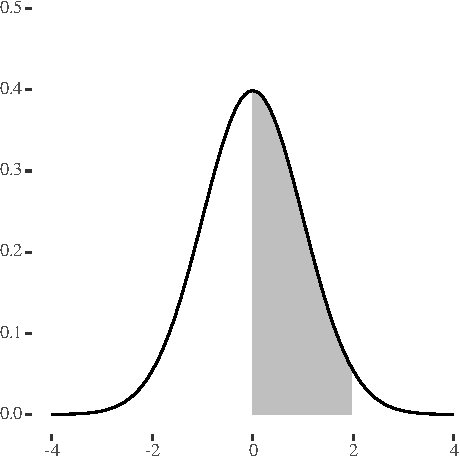
\includegraphics{bxjs_template_files/figure-latex/unnamed-chunk-1-1} 

}

\caption{アイリスデータセット}\label{fig:unnamed-chunk-1}
\end{figure}

\end{document}
